\clearpage

\section{ラズベリーパイになれよう(1)}
\subsection{ファイル、フォルダ}
コンピュータやラズベリーパイの中にあるデータ(音楽、動画、写真、テキストなど)はすべてファイルとして\ruby{扱}{あつか}われています。しばしばファイルには.(ドット)から始まる「\ruby{拡張子}{かくちょうし}」がついており、ファイルがどんな種類なのかを表します。例えば\ruby{画像}{がぞう}の場合は.jpgや動画ファイルの場合はmp4、テキストファイルは.txt、ホームページの場合は.htmlがついています。

ファイルの他にフォルダというものがあります。フォルダはファイルをまとめたものです。ファイルを書類としてフォルダはバインダと考えるとわかりやすいでしょう。フォルダのなかにフォルダをいれることもできます。

\begin{figure}[hb]
  \centering
  \begin{minipage}{0.76\textwidth}
    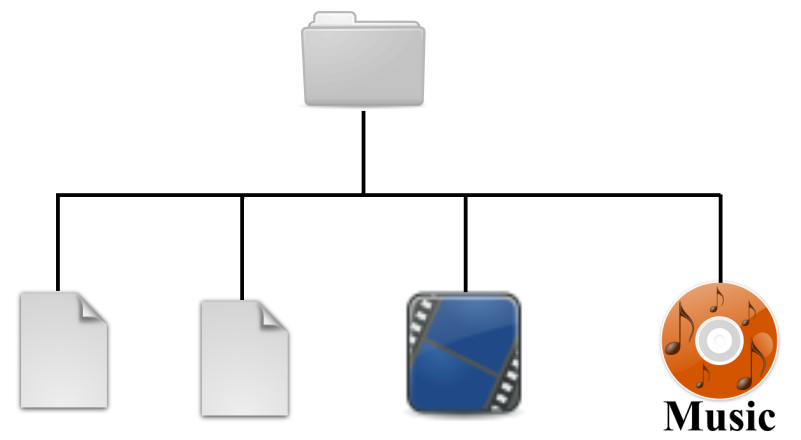
\includegraphics[width=\linewidth]{text01-img/figure15.png}
    \caption{onフォルダ、ファイルの関係}
  \end{minipage}
\end{figure}

%後で修正 上がそろわない
\begin{figure}
  \begin{tabular}{ccc}
    \begin{minipage}{0.33\textwidth}
      \centering
      \textbf{(左)クリック}
      \flushleft
  
      カチッ\\
      \centering
      \raisebox{20mm}{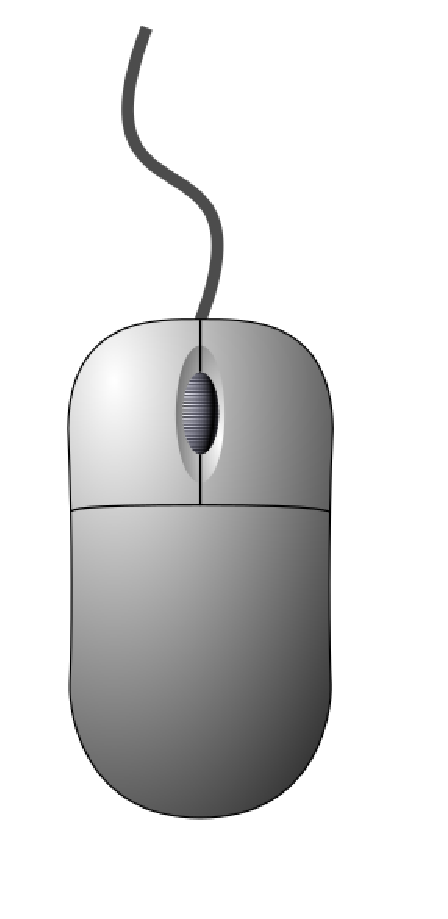
\includegraphics[width=1.651cm,height=3.53cm]{text01-img/textbook-img076.eps}}
  
      \flushleft
      マウスの左側を一度\ruby{押}{お}すこと、アプリなど開きたいときに使おう
    \end{minipage}
  
    \begin{minipage}{0.33\textwidth}
      \centering
      \textbf{ダブルクリック}
      \flushleft
  
      カチカチッ\\
      \centering
      \raisebox{20mm}{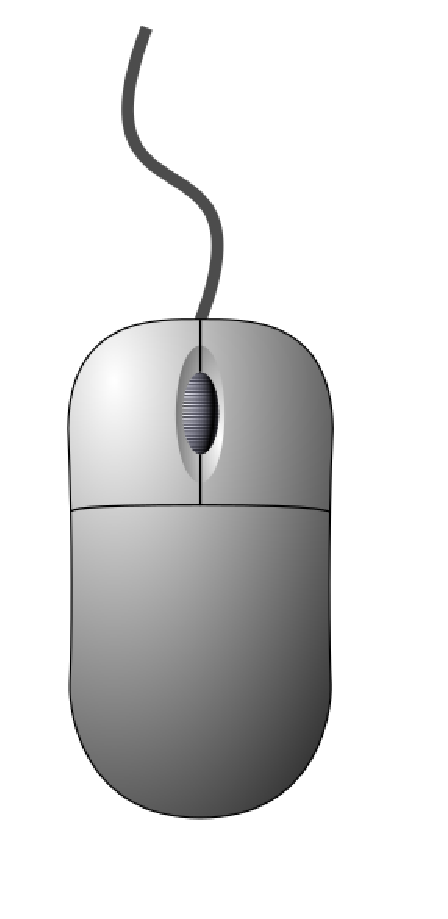
\includegraphics[width=1.651cm,height=3.53cm]{text01-img/textbook-img076.eps}}
  
      \flushleft
      マウスの左側を二回続けて\ruby{押}{お}すこと。 デスクトップのフォルダなどを開くときに使うよ
    \end{minipage}
  
    \begin{minipage}{0.33\textwidth}
      \centering
      \textbf{~~~~~右クリック}
      \flushleft
  
      \hspace{3cm} カチッ\\
      \centering
      \raisebox{20mm}{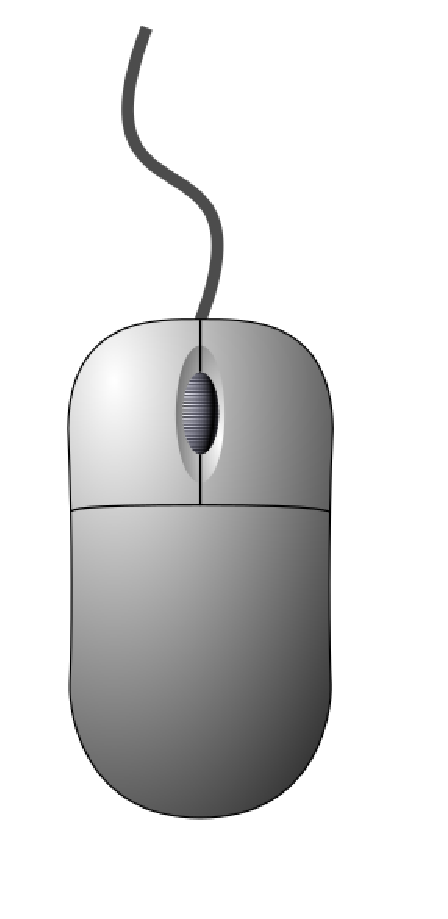
\includegraphics[width=1.651cm,height=3.53cm]{text01-img/textbook-img076.eps}}
  
      \flushleft
      マウスの右側を一度\ruby{押}{お}すこと。メニューなどを\ruby{表示}{ひょうじ}したいときに使うよ
    \end{minipage}
    
  \end{tabular}
\end{figure}
\clearpage



\subsection{例題 1-5 自分のフォルダを\ruby{確認}{かくにん}しよう}
まず、みなさんがこの\ruby{授業}{じゅぎょう}で使う「自分のフォルダ」を\ruby{確認}{かくにん}しましょう。
このとき、注意してもらいたいことが1つあります。
さきほど、みなさんには「ユーザ名」と「パスワード」を\ruby{設定}{せってい}してもらいました。
そのとき\ruby{設定}{せってい}した「ユーザ名」によって、みなさんひとりひとりの「自分のフォルダ」の名前が変わります。
どこが変わるのか、じっさいに見てみましょう。\\

{\bf \large 考え方}\\
\begin{figure}[ht]
  \begin{minipage}{\textwidth}
    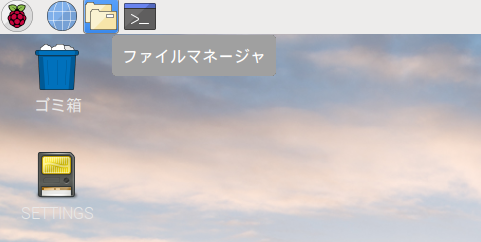
\includegraphics[width=0.4\textwidth]{text01-img/textbook-img032.png}
    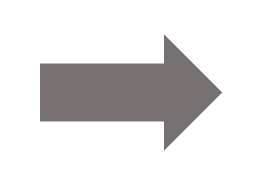
\includegraphics[width=2cm]{text01-img/textbook-img035.png}
    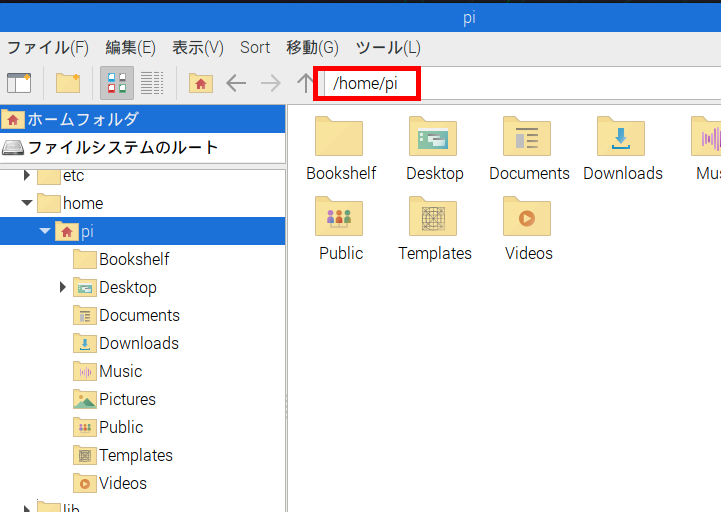
\includegraphics[width=0.5\textwidth]{text01-img/textbook-img1020.png}
  \end{minipage}
  \begin{minipage}{0.4\textwidth}
    1
    ディスプレイの左上の、黄色いアイコンをクリック
  \end{minipage}
  \hspace{2cm}
  \vspace{20pt}
  \begin{minipage}{0.5\textwidth}
    \vspace{20pt}
    2
    ファイルマネージャーが開いて、自分のフォルダが\ruby{表示}{ひょうじ}されます。(ウィンドウの色が\ruby{違}{ちが}うかもしれませんが、色はあとで変えられます)
  \end{minipage}
\end{figure}

\noindent ファイルマネージャーは、初回起動時は自分のフォルダを\ruby{表示}{ひょうじ}します。
この、ファイルマネージャの写真の赤\ruby{枠}{わく}で囲ったところには、自分のフォルダのパスが書いてあります。
パスについての\ruby{詳}{くわ}しい説明は、\ruby{以降}{いこう}の回で出てくるので、今はとりあえずフォルダ、ファイルの「住所」と考えてください。
この\ruby{画像}{がぞう}では、/home/piと書いてあります。ですが、みなさんは\ruby{違}{ちが}うはずです。
\textbf{\color{red}ここに、さいしょに\ruby{設定}{せってい}した「ユーザ名」が反映されます。}
たとえば、「takeshi」というユーザ名を\ruby{設定}{せってい}した場合、この赤\ruby{枠}{わく}の中は、
/home/takeshiになります。
\vspace{20pt}

\noindent \textbf{問題 1-6}\\
自分のフォルダのパス(右上の\ruby{画像}{がぞう}の赤い\ruby{枠}{わく}で囲まれた部分)を、下の\ruby{空欄}{くうらん}に書き写してみよう\\
\vskip\baselineskip
\underline{答え:\hspace{13.5cm}}
\clearpage


\subsection{例題 1-6 フォルダを作成しよう}
Documentsフォルダ直下にtaro、hanako、saburoという名前のフォルダを作成しましょう。\\

{\bf \large 考え方}
\begin{figure}[ht]
  \centering
  \begin{minipage}{0.9\textwidth}
    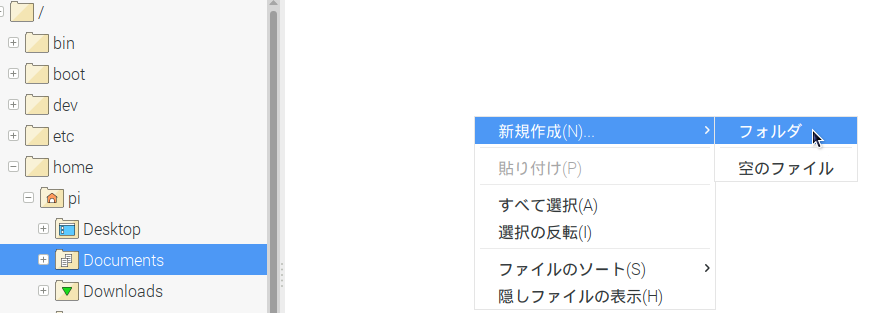
\includegraphics[width=\linewidth]{text01-img/textbook-img034.png}
    1 ファイルマネージャーの空白部分で右クリックし、「New Folder」にカーソルを合わせてクリック
     \vspace{60pt}
  \end{minipage}

  \centering
  \begin{minipage}{0.9\textwidth}
    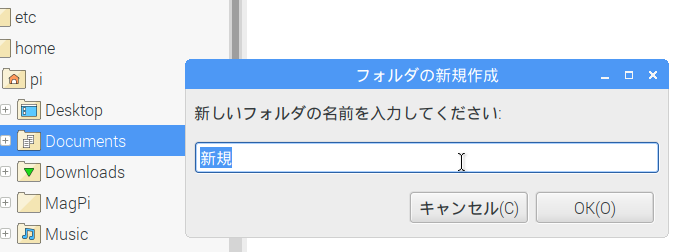
\includegraphics[width=\linewidth]{text01-img/textbook-img036.png}
    2 フォルダ名の入力を求められるので、付けたい名前を入力しよう
  \end{minipage}
\end{figure}
\clearpage




{\bf\large 考え方(続き)}
\begin{figure}[hb]
  \centering
  \begin{minipage}{0.9\textwidth}
  %[Warning: Image ignored] % Unhandled or unsupported graphics:
   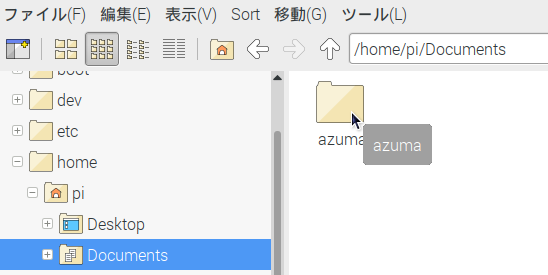
\includegraphics[width=\linewidth]{text01-img/textbook-img038.png}
    3 名前を入力し、OKを\ruby{押}{お}すと上の\ruby{画像}{がぞう}のようにフォルダが作成されます
  \end{minipage}

\end{figure}
\begin{figure}[hb]
  \centering
  \begin{minipage}{0.9\textwidth}
    {	\large
      フォルダは大事です。

      フォルダに、\ruby{画像}{がぞう}やプログラムのコードを\ruby{保存}{ほぞん}しておくので、わかりやすく\ruby{関係性}{かんけいせい}のある名前を付けてあげましょう
      \vskip.5\baselineskip
      ファイルやフォルダの名前は、空白の入らない半角ローマ字にしておくと、後でプログラムから使う時に便利だよ
    }
  \end{minipage}
\end{figure}
\clearpage

\begin{figure}[ht]
  \flushleft{\bf\large 答え}
  \vspace{8mm}\\
  \centering
  \begin{minipage}{0.8\textwidth}
   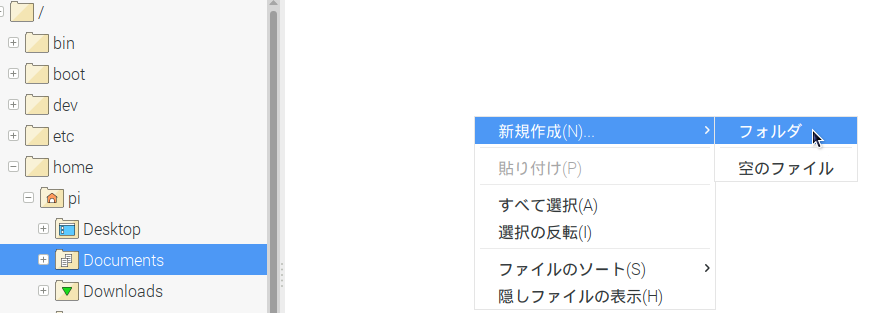
\includegraphics[width=\linewidth]{text01-img/textbook-img034.png}
    1
    \ 左上のフォルダアイコンをクリックし

    フォルダマネージャー上で右クリックし、上の\ruby{画像}{がぞう}のようにしよう
  \end{minipage}
  \vspace{\baselineskip}

  \centering
  %[Warning: Image ignored] % Unhandled or unsupported graphics:
  \begin{minipage}{0.8\textwidth}
   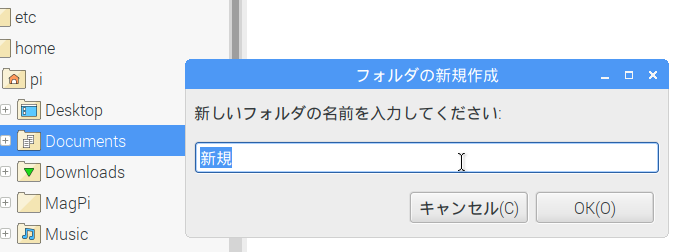
\includegraphics[width=\linewidth]{text01-img/textbook-img036.png}
    2
    \ 「New Folder」を選び、名前\ruby{設定}{せってい}に行こう
  \end{minipage}
  \vspace{\baselineskip}

  \centering
  %[Warning: Image ignored] % Unhandled or unsupported graphics:
  \begin{minipage}{0.8\textwidth}
  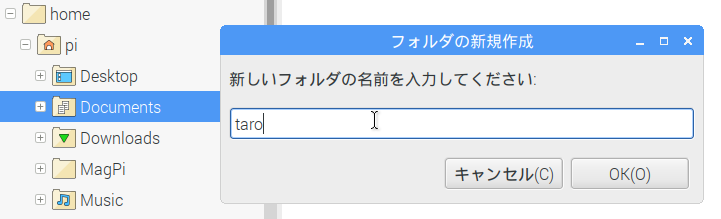
\includegraphics[width=\linewidth]{text01-img/textbook-img039.png}
    3
    \ taroと名前を入力し、OKを\ruby{押}{お}す
  \end{minipage}
  \vspace{\baselineskip}

  \centering
  %[Warning: Image ignored] % Unhandled or unsupported graphics:
  \begin{minipage}{0.8\textwidth}
  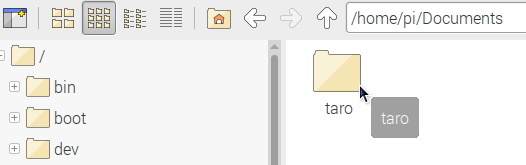
\includegraphics[width=\linewidth]{text01-img/textbook-img040.png}
    4
    \ taroというフォルダを作成できていることを\ruby{確認}{かくにん}しよう
  \end{minipage}

\end{figure}
\clearpage



\begin{figure}
  \flushleft{\bf\large
    答え(続き)}\\
  \vspace{10mm}
  \centering
  %[Warning: Image ignored] % Unhandled or unsupported graphics:
  \begin{minipage}{0.8\textwidth}
  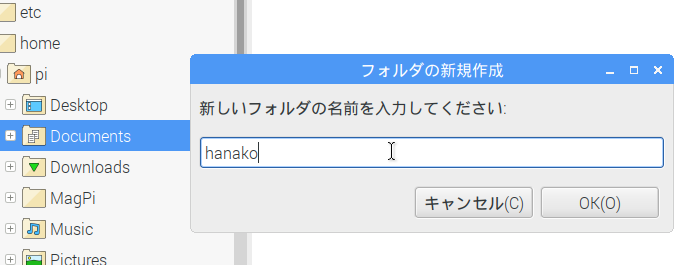
\includegraphics[width=\linewidth]{text01-img/textbook-img041.png}
    5
    \ 先ほどと同じように右クリックから「New Folder」を選び、hanakoという名前でフォルダを作成
  \end{minipage}
  \vspace{\baselineskip}

  \centering
  %[Warning: Image ignored] % Unhandled or unsupported graphics:
  \begin{minipage}{0.8\textwidth}
  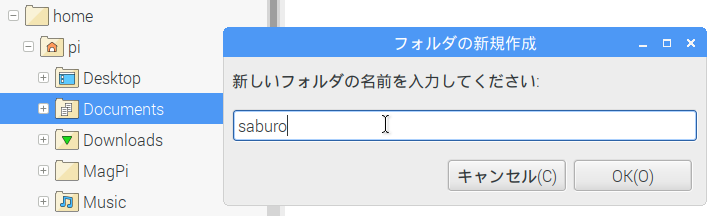
\includegraphics[width=\linewidth]{text01-img/textbook-img042.png}
    6
    \ saburoというフォルダを先ほどと同じ方法で作成
  \end{minipage}
  \vspace{\baselineskip}

  \centering
  %[Warning: Image ignored] % Unhandled or unsupported graphics:
  \begin{minipage}{0.8\textwidth}
  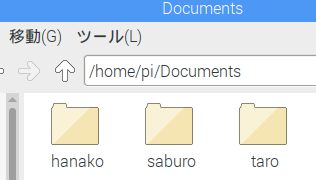
\includegraphics[width=\linewidth]{text01-img/textbook-img043.png}
    7 
    \ taro , hanako , saburoのフォルダが作成されていることを\ruby{確認}{かくにん}してみよう
  \end{minipage}
  \vspace{10mm}
  \flushleft

  \noindent \textbf{問題 1-7}\\
  例題と同じ方法で、akahoshi、imaoka、hamanakaという名前のフォルダを作ろう
  % \refstepcounter{Question}\theQuestion\label{Q:hasAnswer02-1}

  % 例題と同じ方法で、akahoshi、imaoka、hamanakaという名前のフォルダを作ろう

\end{figure}
\clearpage


% \subsection{例題 1-7 フォルダを\ruby{移動}{いどう}しよう}
% Desktop直下に「space1」と「space2」を作り、「space1」の中に「move」フォルダを作り、「move」フォルダを「space2」に\ruby{移動}{いどう}しよう

% \flushleft{\bf\large 考え方}

\begin{figure}[htbp]
  \subsection{例題 1-7 フォルダを\ruby{移動}{いどう}しよう}
  Desktop直下に「space1」と「space2」を作り、「space1」の中に「move」フォルダを作り、「move」フォルダを「space2」に\ruby{移動}{いどう}しよう

  \flushleft{\bf\large 考え方} 
  \centering
  %[Warning: Image ignored] % Unhandled or unsupported graphics:
  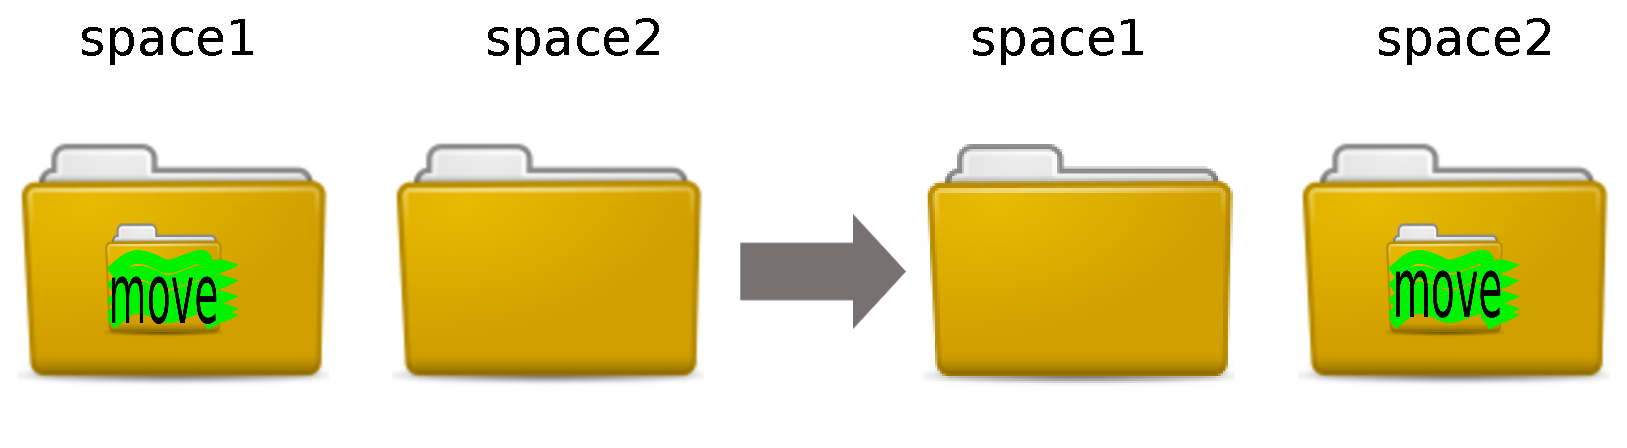
\includegraphics[width=0.8\textwidth]{text01-img/fig15-1.eps}
  \begin{minipage}{15.297cm}
    フォルダやファイルは後からでも動かすことができるよ。
  \end{minipage}

  % \begin{minipage}{5.963cm}
  \begin{minipage}{0.4\textwidth}
    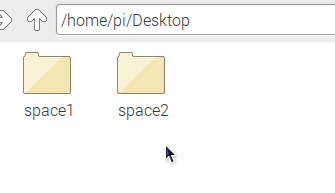
\includegraphics[width=\linewidth]{text01-img/textbook-img051.png}
    {\flushleft
      1 左側のDesktopをクリックし、space1とspace2を作成
    }
  \end{minipage}
  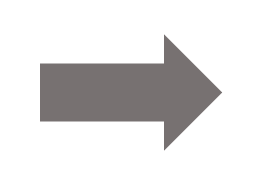
\includegraphics[width=2cm]{text01-img/textbook-img052.png}
  \begin{minipage}{0.4\textwidth}
    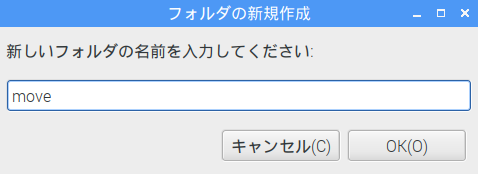
\includegraphics[width=\linewidth]{text01-img/textbook-img050.png}
    {\flushleft
      2 space1の中にmoveフォルダを作成
    }
  \end{minipage}

  \centering
  \begin{minipage}{0.4\textwidth}
    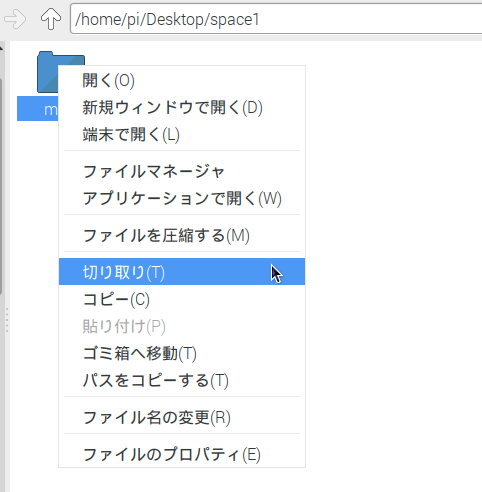
\includegraphics[width=\linewidth]{text01-img/textbook-img048.png}
    {\flushleft
      3 moveフォルダ上で右クリックし、切り取りをクリック
    }
  \end{minipage}
  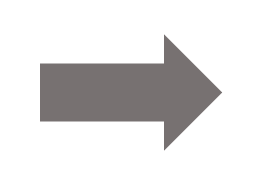
\includegraphics[width=2cm]{text01-img/textbook-img049.png}
  \begin{minipage}{0.4\textwidth}
    %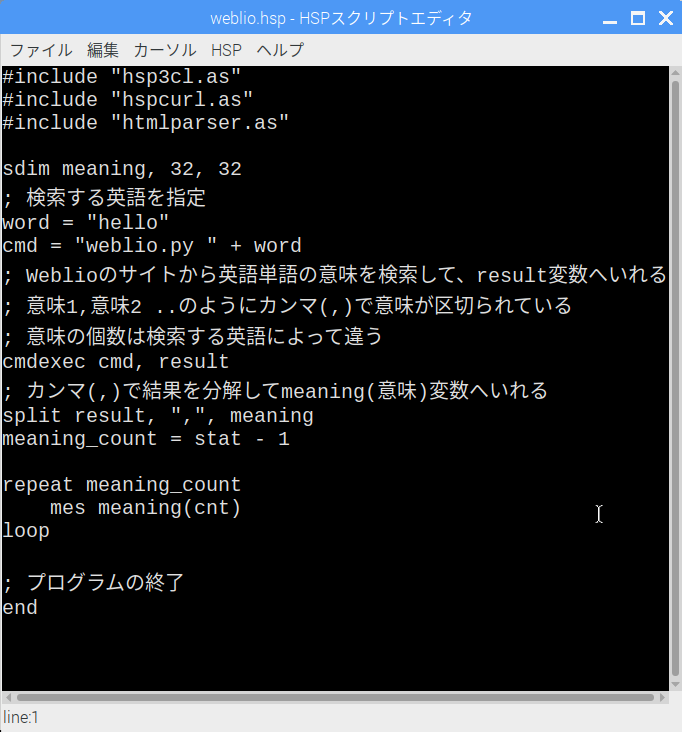
\includegraphics[width=2.168cm,height=1.542cm]{textbook-img047.png}
    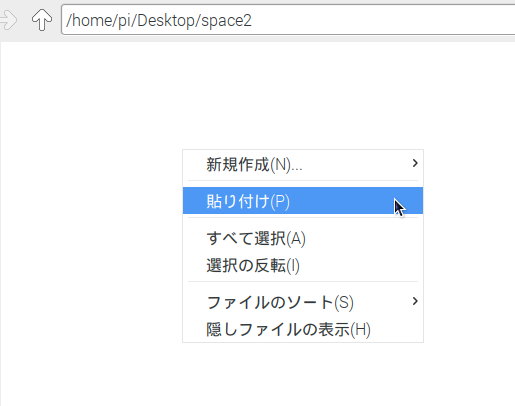
\includegraphics[width=\linewidth]{text01-img/textbook-img046.png}
    {\flushleft
      4 space2の中で右クリック、\ruby{貼}{は}り付けをクリック
    }
  \end{minipage}

  %[Warning: Image ignored] % Unhandled or unsupported graphics:
  \begin{minipage}{6.589cm}
    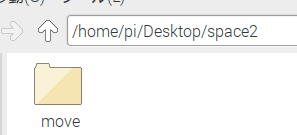
\includegraphics[width=7.218cm]{text01-img/textbook-img045.png}
    {\flushleft
      5 space1の中にあったmoveフォルダがspace2に\ruby{移動}{いどう}しました
    }
  \end{minipage}

  \flushleft
  \noindent \textbf{問題 1-8}\\
  「space1」フォルダ内に「rasp」フォルダを作り、さらにそのフォルダ内に「berry」フォルダを作成して「rasp」フォルダを「space2」フォルダに\ruby{移動}{いどう}させよう。そして中身を\ruby{確認}{かくにん}しよう
  
\end{figure}

\clearpage


\subsection{例題 1-8 ファイル名を\ruby{変更}{へんこう}しよう}
\noindent「before」という名前のフォルダをDocuments直下に1つ作り、その作成した後でフォルダ名を「after」に変えよう

\begin{figure}[ht]
  \flushleft{\bf\large 考え方}

  \centering
  %[Warning: Image ignored] % Unhandled or unsupported graphics:
  \begin{minipage}{1.978cm}
    
\includegraphics[width=1.5cm]{text01-img/textbook-img044.png}
    frog
  \end{minipage}
  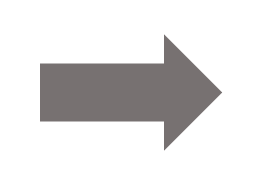
\includegraphics[width=2cm]{text01-img/textbook-img052.png}
  \begin{minipage}{1.978cm}
    
\includegraphics[width=1.5cm]{text01-img/textbook-img044.png}
    dog
  \end{minipage}
  \begin{minipage}{6.319cm}
    まちがったフォルダ名をつけたとき、名前を変えたいときなどに使います。
  \end{minipage}

  \begin{minipage}{0.4\textwidth}
    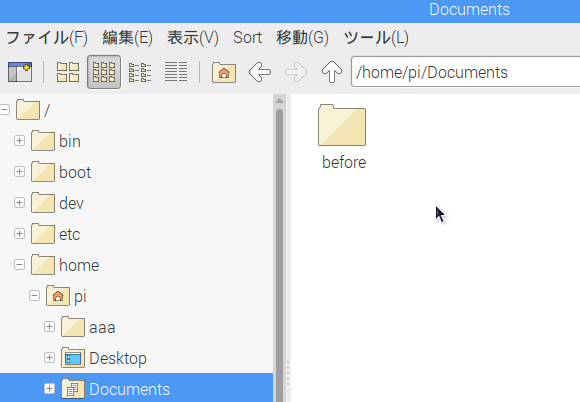
\includegraphics[width=\linewidth]{text01-img/textbook-img058.png}
    \flushleft
    1 左側のDocumentsをクリックし「before」フォルダを作成
  \end{minipage}
  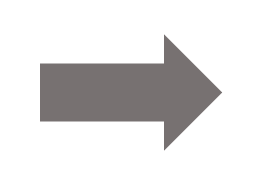
\includegraphics[width=2cm]{text01-img/textbook-img052.png}
  \begin{minipage}{0.4\textwidth}
    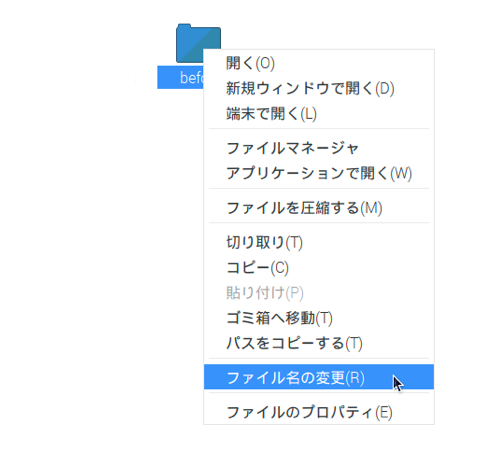
\includegraphics[width=\linewidth]{text01-img/textbook-img057.png}
    \flushleft
    2 フォルダ上で右クリックし、

    ファイル名の\ruby{変更}{へんこう}をクリック
  \end{minipage}
  %[Warning: Image ignored] % Unhandled or unsupported graphics:

  \begin{minipage}{0.4\textwidth}
    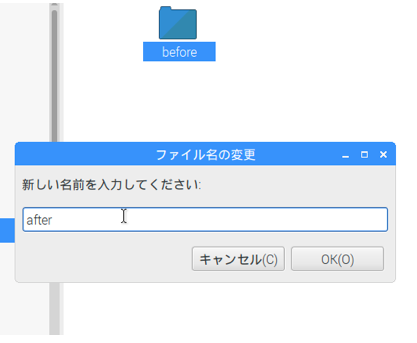
\includegraphics[width=\linewidth]{text01-img/textbook-img055.png}
    3 名前を「after」に\ruby{変更}{へんこう}

    OKをクリック
  \end{minipage}
  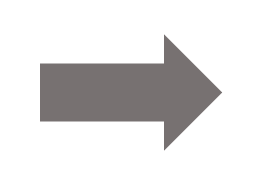
\includegraphics[width=2cm]{text01-img/textbook-img053.png}
  \begin{minipage}{0.4\textwidth}
    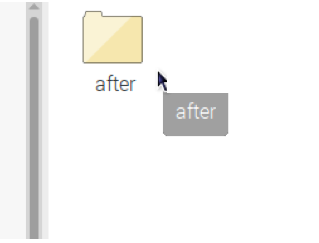
\includegraphics[width=\linewidth]{text01-img/textbook-img056.png}
    4 変更を\ruby{確認}{かくにん}
  \end{minipage}
  \centering

  \begin{minipage}{5.751cm}
    フォルダ名の\ruby{変更}{へんこう}は、よく使うので覚えておこう
  \end{minipage}

  \flushleft
  \noindent \textbf{問題 1-9}\\
  miss\_name」という名前のフォルダを1つ作り、その作成した後でフォルダ名を「success\_name」に変えよう

\end{figure}


\clearpage

\begin{figure}[ht]
  \subsection{例題 1-9 日本語入力と英字入力について}
  \flushleft
  Mousepadを開き、アルファベットをa〜zまで入力しよう。その後「こんにちは」「こんばんは」「ごきげんよう」「さようなら」「ありがとう」をそれぞれ一行に入力しましょう。
  
  {\bf\large 考え方}

  \centering
  \begin{minipage}{\textwidth}
    % 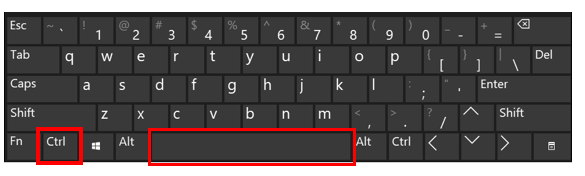
\includegraphics[width=0.4\textwidth]{text01-img/textbook-img065.png}
    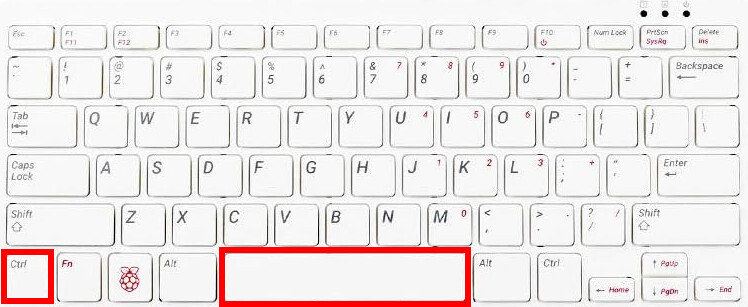
\includegraphics[width=0.4\textwidth]{text01-img/2024_keyboard.jpg}
    \raisebox{10mm}
    {
      \begin{minipage}{0.5\textwidth}
        赤わくで囲んだCtrlとスペースを同時に\ruby{押}{お}すことで
        英字入力と日本語入力を切り\ruby{替}{か}えることができるよ
      \end{minipage}
    }
  \end{minipage}

  \begin{minipage}{0.3\textwidth}
    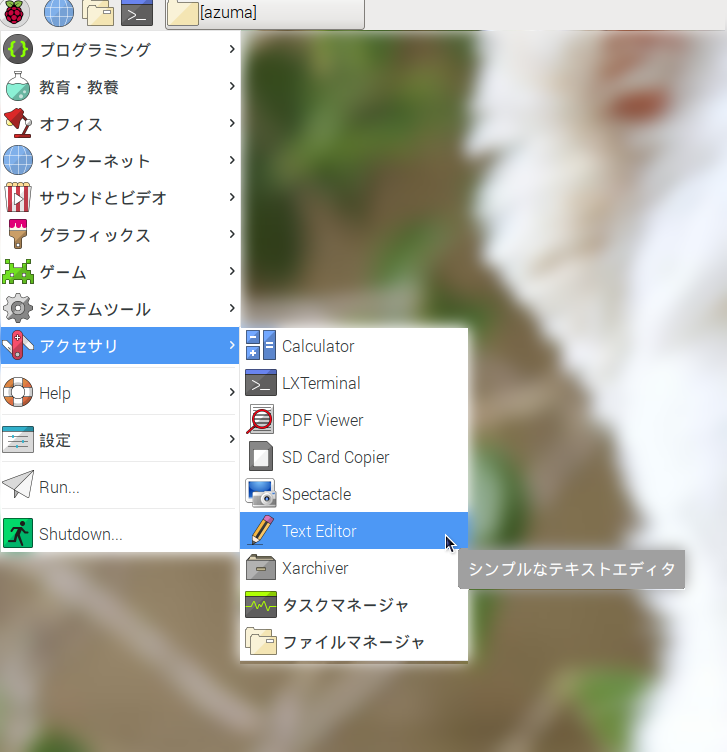
\includegraphics[width=\linewidth]{text01-img/textbook-img064.png}
    \flushleft
    1 ラズベリーのアイコンをクリックしてアクセサリー>Text editorを開こう
  \end{minipage}
  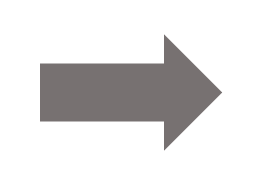
\includegraphics[width=2cm]{text01-img/textbook-img053.png}
  \begin{minipage}{0.4\textwidth}
    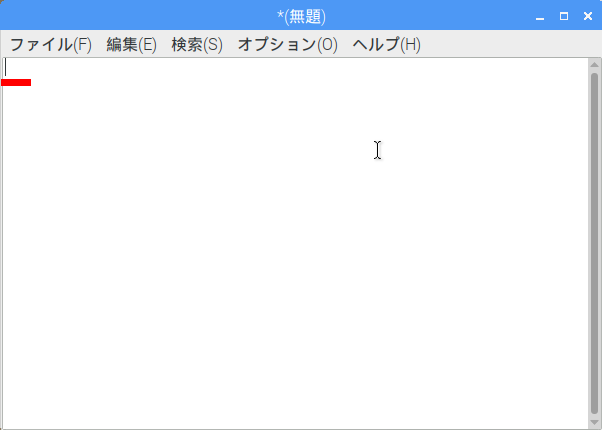
\includegraphics[width=\linewidth]{text01-img/textbook-img063.png}
    \flushleft
    2 赤線が引かれているところをクリックしてテキストエディタにカーソル(\ruby{縦棒}{たてぼう})が入っていることを\ruby{確認}{かくにん}してください。
  \end{minipage}

  \begin{minipage}{0.4\textwidth}
    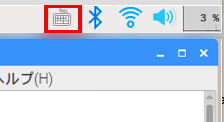
\includegraphics[width=\linewidth]{text01-img/textbook-img059.png}
    \flushleft
    3 Ctrlとスペースキーを同時に\ruby{押}{お}して

    英字入力に切り\ruby{替}{か}えよう。アイコンがキーボードであることを\ruby{確認}{かくにん}しよう。
  \end{minipage}
  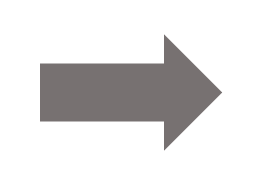
\includegraphics[width=2cm]{text01-img/textbook-img053.png}
  \begin{minipage}{0.4\textwidth}
    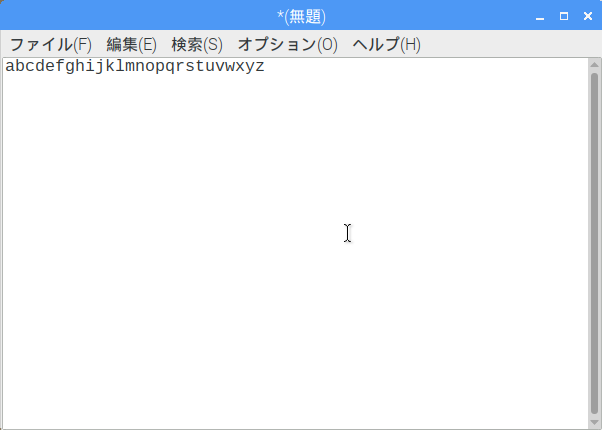
\includegraphics[width=\linewidth]{text01-img/textbook-img061.png}
    \flushleft
    4 英字入力でa〜zまで入力しよう
  \end{minipage}

  \begin{minipage}{0.4\textwidth}
    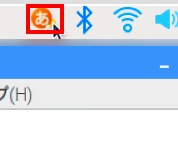
\includegraphics[width=\linewidth]{text01-img/textbook-img062.png}
    \flushleft
    5 Ctrlとスペースキーを同時に\ruby{押}{お}して
    アイコンが“あ”になったか\ruby{確認}{かくにん}しましょう。
  \end{minipage}
  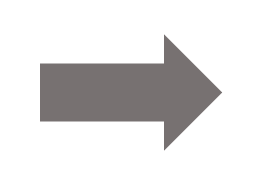
\includegraphics[width=2cm]{text01-img/textbook-img053.png}
  \begin{minipage}{0.4\textwidth}
    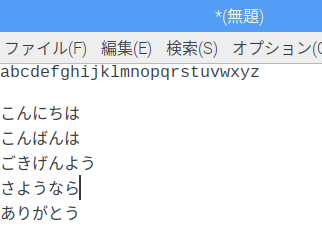
\includegraphics[width=\linewidth]{text01-img/textbook-img060.png}
    \flushleft
    6 こんにちは〜ありがとうを入力\\
    7 完成
  \end{minipage}
  
  \flushleft
  \noindent \textbf{問題 1-10}\\
  Text editorでA〜Zを入力しよう
  \noindent ヒント 
  英字入力時にshiftキーを\ruby{押}{お}しながらアルファベットキーを打つと大文字で入力できます
\end{figure}



\clearpage


\begin{figure}
  \subsection{例題 1-10 半角入力と全角入力について}
  Text Editorを開き、半角入力でアルファベットをa〜zまで入力し、その後、全角入力で
  アルファベットa〜zまで入力しよう。全角と半角文字の\ruby{違}{ちが}いを\ruby{理解}{りかい}しよう。

  {\bf\large 考え方}

  \centering
  %[Warning: Image ignored] % Unhandled or unsupported graphics:
  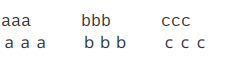
\includegraphics[width=5.978cm]{text01-img/textbook-img066.png}
  \raisebox{8mm}{
    \begin{minipage}{6.762cm}
      {文字が小さいのが半角}\\
      {文字が大きいのが全角}
    \end{minipage}
  }

  \begin{minipage}{16.578cm}
    % \bigskip
    アルファベットのサイズからも分かる通り、大きいサイズが全角で、小さいサイズが半角だと覚えておくといいよ
  \end{minipage}

  \begin{minipage}{0.3\textwidth}
    %[Warning: Image ignored] % Unhandled or unsupported graphics:
    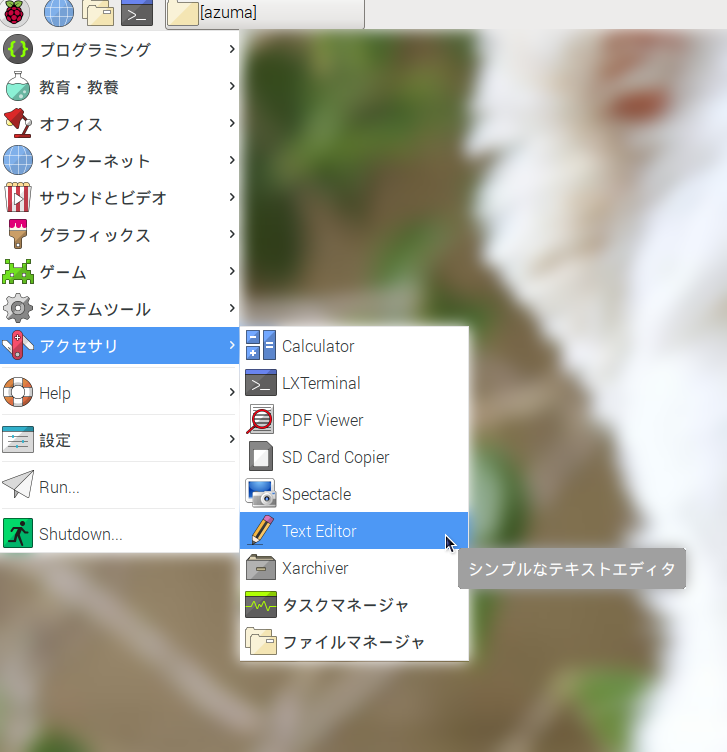
\includegraphics[width=\linewidth]{text01-img/textbook-img067.png}
    \flushleft
    1 Text editorを開こう
  \end{minipage}
  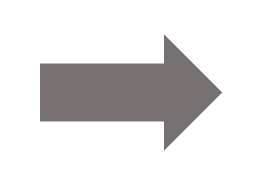
\includegraphics[width=2cm]{text01-img/textbook-img073.png}
  \begin{minipage}{0.3\textwidth}
    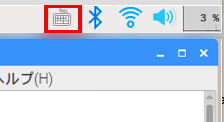
\includegraphics[width=\linewidth]{text01-img/textbook-img059.png}
    \flushleft
    2 キーボードのアイコンになっていることを\ruby{確認}{かくにん}して半角を入力しよう
  \end{minipage}

  \begin{minipage}{0.3\textwidth}
    \includegraphics[width=\linewidth]{text01-img/textbook-img059.png}
    \flushleft
    3 半角のアルファベットを入力し終えたら右上のキーボードアイコンをクリック
  \end{minipage}
  \includegraphics[width=2cm]{text01-img/textbook-img073.png}
  \begin{minipage}{0.3\textwidth}
    \includegraphics[width=\linewidth]{text01-img/textbook-img062.png}
    \flushleft
    4 アイコンが変わったことを\ruby{確認}{かくにん}しよう
  \end{minipage}

  \begin{minipage}{0.3\textwidth}
    \includegraphics[width=\linewidth]{text01-img/textbook-img069.png}
    \flushleft
    5 アイコンを右クリックして、全角英数を\ruby{選択}{せんたく}
  \end{minipage}
  \includegraphics[width=2cm]{text01-img/textbook-img073.png}
  \begin{minipage}{0.3\textwidth}
    \includegraphics[width=\linewidth]{text01-img/textbook-img070.png}
    \flushleft
    6 入力
  \end{minipage}

  \vspace{3mm}
  \begin{minipage}{\textwidth}
    {\centering\textbf{\color{red}{
      プログラミングでアルファベット,記号を入力するときは
      半角(小さい文字)で入力しましょう}}
    }
  \end{minipage}

  \flushleft
  \noindent \textbf{問題1-11}\\
  Text editorで半角A〜Zと全角A〜Zを入力しよう
  ヒント

  英字入力時にshiftキーを\ruby{押}{お}しながらアルファベットキーを打つと大文字で入力できます

\end{figure}
\clearpage


\begin{figure}[t]
  \subsection{例題 1-11 ブラウザでけんさくをしよう}
  ブラウザを開いてけんさくをしよう。ブラウザを使用するとウェブサイトを開くことができます。もし、困ったことがあったら自分でけんさくをできるように使い方を覚えておきましょう。
  \vskip.5\baselineskip
  \subsection{ブラウザ立ち上げとマウスそうさについて}
  ブラウザを立ち上げ、好きなものを調べよう

  {\bf\large 考え方}

  \begin{minipage}{\textwidth}
    \begin{minipage}{0.45\textwidth}
      \includegraphics[width=\linewidth]{text01-img/textbook-img071.png}
      1 デスクトップの左上のアイコンを左クリック
    \end{minipage}
    \includegraphics[width=1.505cm]{text01-img/textbook-img073.png}
    \begin{minipage}{0.45\textwidth}
      \includegraphics[width=\linewidth]{text01-img/textbook-img075.png}
      2 ブラウザが立ち上がり、赤で囲われている部分を左クリック
    \end{minipage}
  \end{minipage}

  \hfill\begin{minipage}{0.45\textwidth}
    {\centering
      \includegraphics[width=1.707cm]{text01-img/textbook-img074.png}
    }\\
    \includegraphics[width=\linewidth]{text01-img/textbook-img072.png}
    3 キーボードでけんさくしたいワードを入力しよう。入力し終えたらenterキーを\ruby{押}{お}そう
  \end{minipage}

  \vspace{70mm}

\end{figure}
\clearpage


\begin{figure}
  \subsubsection{図~\ref{fig:20}のように赤い四角で囲われているところにけんさくしたい言葉を入れてエンターキーを\ruby{押}{お}すとけんさくができます。例えば”ねこ”とけんさくしてみましょう。}
  \centering
  \includegraphics[width=0.45\textwidth]{text01-img/textbook-img077.png}
  \caption{けんさくバー}\label{fig:20}
  
  \flushleft
  けんさくすると図~\ref{fig:21}このような感じになります。青線で囲んであるところは今けんさくした言葉です。赤線で囲われている\textbf{\ruby{画像}{がぞう}}をクリックすると\ruby{画像}{がぞう}をけんさくできます。クリックしてみましょう。


  \centering
  \includegraphics[width=0.45\textwidth]{text01-img/textbook-img078.png}
  \caption{”ねこ”けんさく結果\\
  けんりの関けいで\ruby{画像}{がぞう}をぼかしてあります}\label{fig:21}
  \flushleft
  図~\ref{fig:22}のように”ねこ”の\ruby{画像}{がぞう}がたくさんでてきました。
  \textbf{すべて}をクリックすると先ほどの~\ref{fig:20}のようなホームページけんさくに\ruby{戻}{もど}れます。


  \centering
  \includegraphics[width=0.45\textwidth]{text01-img/textbook-img079.png}
  \caption{”ねこ”\ruby{画像}{がぞう}けんさく結果}\label{fig:22}
  \flushleft
  \noindent \textbf{問題 1-12}\\
  自分の好きなキーワードをけんさくしてみよう

\end{figure}
\clearpage



\begin{figure}[t]
  \subsection{例題 1-12 キーボード入力の練習をしよう}
  ブラウザで”Etyping”とけんさくし、キーボードタイピングサイトでタイピングに\ruby{慣}{な}れよう

  \textbf{考え方}\\
  \textbf{タイピング} ・・・キーボードで文字を入力すること
  \vskip.5\baselineskip
  \begin{minipage}{\textwidth}
    \raisebox{30mm}{
      \begin{minipage}{0.65\textwidth}
        パソコンでの文字入力はローマ字入力が\ruby{基本}{きほん}です。
        けんさくなどをしたいとき、キーボードで文字を入力します。
        今回はタイピング練習サイト”Etyping”でタイピングを
        練習しましょう。

        \includegraphics[width=0.7\linewidth]{text01-img/textbook-img081.png}
        \includegraphics[width=0.25\linewidth]{text01-img/textbook-img082.png}
      \end{minipage} }
    \includegraphics[width=0.3\textwidth]{text01-img/textbook-img080.png}
  \end{minipage}

  \centering

  {\centering
    \textbf{まずはタイピングゲームを開こう}
    \par}

  \centering

  \begin{minipage}{0.4\textwidth}
    \includegraphics[width=\linewidth]{text01-img/textbook-img071.png}
    1 左上のアイコンをクリックしよう
  \end{minipage}
  \includegraphics[width=2cm]{text01-img/textbook-img084.png}
  \begin{minipage}{0.4\textwidth}
    \includegraphics[width=\linewidth]{text01-img/textbook-img083.png}
    2 けんさくらんに”Etyping”と入力しenterを\ruby{押}{お}そう
  \end{minipage}
  \vskip.5\baselineskip
  \begin{minipage}{0.45\textwidth}
    \includegraphics[width=\linewidth]{text01-img/textbook-img086.png}
    3 サイトに入りましょう。赤わくで囲われているところのうち、一番上の「インターネットでタイピング練習 イータイピング」をクリックします。
  \end{minipage}
  \begin{minipage}{0.45\textwidth}
    \includegraphics[width=\linewidth]{text01-img/textbook-img085.png}
    赤線で線が引かれているところ、黒い四角で囲んであるアイコンをよく確かめてください。
  \end{minipage}

  \centering

\end{figure}

\clearpage

\begin{figure}
  \textbf{考え方(続き)}

  \centering
  \includegraphics[width=0.7\textwidth]{text01-img/textbook-img087.png}
  \begin{minipage}{0.7\textwidth}
    4 ホームページが開けたら黒で囲んである\textbf{今すぐチェック!}をクリックしよう

  \end{minipage}
\end{figure}





\begin{figure}
  \centering
  \includegraphics[width=0.7\textwidth]{text01-img/textbook-img088.png}

  \begin{minipage}{0.7\textwidth}
    5 黒い四角で囲んである\textbf{今すぐチェック!}をもう一度クリックします。
  \end{minipage}
\end{figure}

\clearpage



\begin{figure}[t]
  \subsection{ 考え方(続き)}

  \centering
  \includegraphics[width=	0.6\textwidth]{text01-img/textbook-img091.png}
  \raisebox{40mm}{\begin{minipage}{5cm}
      6 黒い四角で囲んである
      \textbf{スタート}を
      クリックします。
    \end{minipage}
  }

  \bigskip
  \includegraphics[width=0.6\textwidth]{text01-img/textbook-img090.png}
  \raisebox{40mm}{\begin{minipage}{5cm}
      7 キーボードのスペースキーを\ruby{押}{お}すとゲームがスタートします。


      \bigskip
    \end{minipage}
  }

  \bigskip


  \bigskip

  \includegraphics[width=0.6\textwidth]{text01-img/textbook-img089.png}
  \raisebox{30mm}{\begin{minipage}{5cm}
      8 ゲームでは黒で囲んである文字をキーボードで入力します。


      \bigskip

      キーの位置は画面にオレンジで色がついています。


      \bigskip

      \ruby{慣}{な}れてきたら、オレンジになっている指でキーボードを\ruby{押}{お}せるように練習してみましょう。


      \bigskip
    \end{minipage}
  }

  \bigskip
  \bigskip
  \bigskip
  \bigskip
\end{figure}
\clearpage



\begin{figure}[t]
  \subsection{例題 1-13 \ruby{画像}{がぞう}けんさくし、\ruby{画像}{がぞう}を\ruby{保存}{ほぞん}しよう}
  Documentsフォルダに自分の名前のフォルダを作り、さらにその中にkuma、usagi、inuフォルダを作成、そのフォルダに\ruby{画像}{がぞう}けんさくで得たクマ、うさぎ、犬の\ruby{画像}{がぞう}をそれぞれ\ruby{対応}{たいおう}するフォルダに\ruby{保存}{ほぞん}しよう

  \textbf{考え方}

  \bigskip
  \centering

    \begin{minipage}{0.4\textwidth}
      \includegraphics[width=\linewidth]{text01-img/textbook-img092.png}
    \end{minipage}
    \includegraphics[width=2cm]{text01-img/textbook-img073.png}
    \begin{minipage}{0.4\textwidth}
      \includegraphics[width=0.5\linewidth]{text01-img/textbook-img044.png}
    \end{minipage}

  \flushleft
  {\bfseries
    フォルダに\ruby{画像}{がぞう}を\ruby{保存}{ほぞん}しよう}

  ブラウザの\ruby{画像}{がぞう}けんさくしたいものはラズベリーパイのフォルダ内に\ruby{保存}{ほぞん}することができる

  \ruby{画像}{がぞう}と関連のあるフォルダ名にしておくと、どのような\ruby{画像}{がぞう}が\ruby{保存}{ほぞん}されているのかわかりやすいよ

  \begin{minipage}{0.4\textwidth}
    \includegraphics[width=\linewidth]{text01-img/textbook-img093.png}
    \flushleft
    1 例題の方法で自分の名前のフォルダをDocuments内に作成しよう
  \end{minipage}
  \includegraphics[width=2cm]{text01-img/textbook-img073.png}
  \begin{minipage}{0.4\textwidth}
    \includegraphics[width=\linewidth]{text01-img/textbook-img094.jpg}
    \flushleft
    2 自分のフォルダをダブルクリックし、その中に上の\ruby{画像}{がぞう}のように3つのフォルダを作成
  \end{minipage}

  \begin{minipage}{0.4\textwidth}
    \includegraphics[width=\linewidth]{text01-img/textbook-img096.png}
    \flushleft
    3 ブラウザを立ち上げてくまをけんさくし、上の\ruby{画像}{がぞう}の赤色で囲われた”\ruby{画像}{がぞう}”をクリック
  \end{minipage}
  \includegraphics[width=2cm]{text01-img/textbook-img073.png}
  \begin{minipage}{0.4\textwidth}
    \includegraphics[width=\linewidth]{text01-img/textbook-img095.png}
    \flushleft
    4 \ruby{画像}{がぞう}けんさくで好きな\ruby{画像}{がぞう}上で右クリックをし”名前をつけて\ruby{保存}{ほぞん}”をクリック
  \end{minipage}

\end{figure}

\clearpage

\begin{figure}[t]
  \flushleft
  \textbf{考え方(続き)}

  \centering

  \begin{minipage}{0.4\textwidth}
    \includegraphics[width=\linewidth]{text01-img/textbook-img097.png}
    \flushleft
    5 \ 名前を\ruby{変更}{へんこう}
  \end{minipage}
  \includegraphics[width=2cm]{text01-img/textbook-img073.png}
  \begin{minipage}{0.4\textwidth}
    \includegraphics[width=\linewidth]{text01-img/textbook-img098.png}
    \flushleft
    6 \ 自分の名前フォルダをダブルクリック
  \end{minipage}

  \bigskip

  \begin{minipage}{0.4\textwidth}
    \includegraphics[width=\linewidth]{text01-img/textbook-img100.png}
    \flushleft
    7 \ “kuma”フォルダをダブルクリック
  \end{minipage}
  \includegraphics[width=2cm]{text01-img/textbook-img073.png}
  \begin{minipage}{0.4\textwidth}
    \includegraphics[width=\linewidth]{text01-img/textbook-img099.png}
    \flushleft
    8 \ 名前と\ruby{保存}{ほぞん}場所が決まったら右下の\ruby{保存}{ほぞん}をクリック
  \end{minipage}

  \bigskip

  \begin{minipage}{0.4\textwidth}
    \includegraphics[width=\linewidth]{text01-img/textbook-img102.png}
    \flushleft
    9 \ kumaフォルダを開き、\ruby{画像}{がぞう}が\ruby{保存}{ほぞん}されているか、\ruby{確認}{かくにん}しよう
  \end{minipage}
  \includegraphics[width=2cm]{text01-img/textbook-img073.png}
  \begin{minipage}{0.4\textwidth}
    \includegraphics[width=\linewidth]{text01-img/textbook-img101.png}
    \flushleft
    10 うさぎで検索し好きな\ruby{画像}{がぞう}を\ruby{保存}{ほぞん}しよう
  \end{minipage}

  \vspace{60mm}

\end{figure}

\bigskip

\clearpage

\begin{figure}[t]
  \textbf{考え方(続き)}

  \begin{minipage}{0.4\textwidth}
    \includegraphics[width=\linewidth]{text01-img/textbook-img103.png}
    \flushleft
    11 同じように\ruby{保存}{ほぞん}フォルダと名前を決めて\ruby{保存}{ほぞん}しよう
  \end{minipage}
  \includegraphics[width=2cm]{text01-img/textbook-img073.png}
  \begin{minipage}{0.4\textwidth}
    \includegraphics[width=\linewidth]{text01-img/textbook-img092.png}
    \flushleft
    12 犬も同様
  \end{minipage}

  \bigskip

  \begin{minipage}{0.4\textwidth}
    \includegraphics[width=\linewidth]{text01-img/textbook-img105.png}
    \flushleft
    13 犬も同様
  \end{minipage}
  \includegraphics[width=2cm]{text01-img/textbook-img073.png}
  \begin{minipage}{0.4\textwidth}
    \includegraphics[width=\linewidth]{text01-img/textbook-img104.png}
    \flushleft
    14 ruby{保存}{ほぞん}成功
  \end{minipage}

  \centering
\end{figure}

\bigskip

\noindent \textbf{問題 1-13}\\
自分の好きなものの\ruby{画像}{がぞう}を\ruby{保存}{ほぞん}し、自分で作成したフォルダに入れよう。

\clearpage

\begin{figure}
  \subsection{がめんの見た目を自分の好きなものに変えよう}
  
  \subsection{例題 1-14 かべ紙を変えよう}
  \ruby{保存}{ほぞん}した\ruby{画像}{がぞう}をデスクトップのかべ紙にしよう

  \textbf{考え方}
  \bigskip

  \centering
  \begin{minipage}{\textwidth}
    デスクトップのかべ紙は変えることができるよ
    いつも目に入るものだから、自分好みにカスタマイズして気分良く勉強できる\ruby{環境}{かんきょう}にしよう
  \end{minipage}

  \begin{minipage}{0.4\textwidth}
    \includegraphics[width=\linewidth]{text01-img/textbook-img107.png}
    \flushleft
    1 デスクトップ上で右クリックし、デスクトップの\ruby{設定}{せってい}をクリック
  \end{minipage}
  \includegraphics[width=2cm]{text01-img/textbook-img073.png}
  \begin{minipage}{0.4\textwidth}
    \includegraphics[width=0.4\linewidth]{text01-img/textbook-img082.png}
    \hfill
    \includegraphics[width=0.4\linewidth]{text01-img/textbook-img106.png}
    \includegraphics[width=\linewidth]{text01-img/textbook-img108.png}
    \flushleft
    2 上の\ruby{画像}{がぞう}のようにクリック
  \end{minipage}

  \begin{minipage}{0.4\textwidth}
    \includegraphics[width=\linewidth]{text01-img/textbook-img110.png}
    \flushleft
    3 デスクトップにしたい\ruby{画像}{がぞう}を選ぼう
  \end{minipage}
  \includegraphics[width=2cm]{text01-img/textbook-img073.png}
  \begin{minipage}{0.4\textwidth}
    \includegraphics[width=\linewidth]{text01-img/textbook-img109.png}
    \flushleft
    4 選び終えたらOKをクリック
  \end{minipage}

  \bigskip


  \flushleft
  \begin{minipage}{0.45\textwidth}
    \includegraphics[width=0.85\linewidth]{text01-img/textbook-img111.png}\\
    5 デスクトップが変わっているよ
  \end{minipage}

  \bigskip

  \noindent \textbf{問題 1-14}\\
  デスクトップのかべ紙を好きなものに変えてみよう。\ruby{画像}{がぞう}はブラウザでけんさくしてね
\end{figure}

\bigskip

\clearpage
\begin{figure}
  \subsection{例題 1-15 ウィンドウの色を変えてみよう}

  ウィンドウの色を変えてみよう
  
  \textbf{考え方}
  
  \bigskip
  \centering
  \begin{minipage}{\textwidth}
      ウィンドウの色も、デスクトップと同じように変えることができるよ
  \end{minipage}

  \begin{minipage}{0.4\textwidth}
    \includegraphics[width=\linewidth]{text01-img/textbook-img107.png}
    \flushleft
    1 デスクトップ上で右クリックし、デスクトップの\ruby{設定}{せってい}をクリック
  \end{minipage}
  \includegraphics[width=2cm]{text01-img/textbook-img073.png}
  \begin{minipage}{0.4\textwidth}
    \includegraphics[width=\linewidth]{text01-img/textbook-img1001.png}
    \flushleft
    2 上の{画像}{がぞう}の赤く囲われた「システム」をクリックした後、下の「ハイライト色」をクリック
  \end{minipage}

  \begin{minipage}{0.4\textwidth}
    \includegraphics[width=\linewidth]{text01-img/textbook-img1002.png}
    \flushleft
    3 すきな色を選ぼう
  \end{minipage}
  \includegraphics[width=2cm]{text01-img/textbook-img073.png}
  \begin{minipage}{0.4\textwidth}
    \includegraphics[width=\linewidth]{text01-img/textbook-img1003.png}
    \flushleft
    4 選び終えたら、自動的にウィンドウの色が変わっているよ
  \end{minipage}

  \flushleft
  \noindent \textbf{問題 1-15}\\
  UIを好きな色に変えてみよう。

\end{figure}


\bigskip

\clearpage

